\begin{theorem}[Неравенство Коши--Буняковского]
Пусть $\E\xi^2 < \infty,\; \E\eta^2 < \infty$.\\
Тогда $\E|\xi\eta| < \infty, \E|\xi\eta| \leqslant \sqrt{\E\xi^2 \E\eta^2}$.
\end{theorem}
\begin{proof}
Пусть $\E\xi^2 = 0$. Тогда $P(\xi = 0) = 1, \E|\xi\eta| = 0$ и неравенство выполнено.

Пусть теперь $\E\xi^2 \neq 0,\; \E\eta^2 \neq 0$. Введем отнормированные величины:
\[\widetilde{\xi} = \frac{\xi}{\sqrt{\E\xi^2}}, \; \widetilde{\eta} = \frac{\eta}{\sqrt{\E\eta^2}}.\]
Тогда для них $\E\widetilde{\xi}^2 = 1,\; \E\widetilde{\eta}^2 = 1$, откуда 
\[\E(|\widetilde{\xi}| - |\widetilde{\eta}|)^2 = 2 - 2\E|\widetilde{\xi} \widetilde{\eta}| \geqslant 0 \implies \E|\widetilde{\xi}\widetilde{\eta}| \leqslant 1.\]

Значит, $\E\frac{|\xi\eta|}{\sqrt{\E\xi^2} \sqrt{\E\eta^2}} \leqslant 1.$
\end{proof}
\begin{corollary}
Корелляция случайных величин лежит в интервале $[-1; 1]$.
\end{corollary}
\begin{corollary}
Равенство в неравенстве Коши--Буняковского достигается тогда и только тогда когда \[\E(|\widetilde{\eta}| - |\widetilde{\xi}|)^2 = 0 \Leftrightarrow P(|\widetilde{\eta}| - |\widetilde{\xi}| = 0) = 1.\]
То есть, когда величины линейно зависимы.
\end{corollary}
\begin{corollary}
Корреляция принимает $\pm 1$ когда случайные величины линейно зависимы.
\end{corollary}

\begin{theorem}[Неравенство Маркова]
Пусть есть неотрицательная случайная величина $\xi$ и $ a\in \R,\; a > 0,\; \E\xi < \infty$.
Тогда 
\[P(\xi \geqslant a) \leqslant \frac{\E\xi}{a}\]
\end{theorem}
\begin{proof}
Верно неравенство $\xi \geqslant a \cdot I(\xi \geqslant a)$, следовательно $\E\xi \geqslant \E a I(\xi \geqslant a) = aP(\xi \geqslant a)$. Для получения искомого неравенства достаточно поделить на $a$.
\end{proof}
\begin{theorem}[Неравенство Чебышёва]
Пусть $\E\xi^2 < \infty,\; \varepsilon > 0$. Тогда
\[P(|\xi - \E\xi| > \varepsilon) \leqslant \frac{\D\xi}{\varepsilon^2}\]
\end{theorem}
\begin{proof}
Сводится к неравенству Маркова введением случайной величины $\eta = (\xi - \E\xi)^2$.
\end{proof}

\begin{theorem}[ЗБЧ в фоме Чебышёва]
Пусть $\xi_1, \ldots \xi_n$~--- независимые в совокупности одинаково распределенные случайные величины. А также существуют $\E\xi_i = a,\; \D\xi_i = \sigma^2$. Тогда 
\[P\left(\left| \frac{\xi_1 + \ldots + \xi_n}{n} - a \right| > \varepsilon\right) \to 0, n\to \infty.\]
\end{theorem}

\begin{theorem}[Обобщение ЗБЧ]
Пусть $\xi_1, \ldots \xi_n:\; \forall i\neq j\; cov(\xi_i, \xi_j) = 0$.\\
А также, дисперсия каждой $\xi_i$ ограничена:
\[\exists C\; \forall i\; \D\xi_i \leqslant C.\]
Если положить $S_n = \xi_1 + \ldots \xi_n,\; \varepsilon > 0$ и взять некую последовательность $w_n \to \infty, n \to \infty$, то верно:
\[
P\left(\frac{|S_n - \E S_n|}{\sqrt{n} \cdot w_n} > \varepsilon\right) \to 0, n \to \infty.
\]
\end{theorem}
\begin{proof}
Пользуемся неравенством Чебышёва: 
\begin{align*}
    P\left(\frac{|S_n - \E S_n|}{\sqrt{n} \cdot w_n} > \varepsilon\right) = P(|S_n - \E S_n| > \varepsilon \sqrt{n} \cdot w_n) \leqslant \frac{\D S_n}{\varepsilon^2 n w_n^2}\\ = \frac{\D \xi_1 + \ldots + \D \xi_n}{\varepsilon^2 n w_n^2} \leqslant \frac{Cn}{\varepsilon^2 n w_n^2} = \frac{C}{\varepsilon^2 w_n^2} \to 0.
\end{align*}
\end{proof}
\begin{lemmanote}
ЗБЧ в фоме Чебышёва из обобщения получается если положить $w_n = \sqrt{n}$.
\end{lemmanote}

\begin{theorem}[Неравенство Йенсена]
Пусть $g:\R \to \R$~--- выпуклая бореллевская функция и $\E|\xi| < \infty$. Тогда $\E g(\xi) \geqslant g(\E\xi)$
\end{theorem}
\begin{proof}
Определение выпуклости:
\[\forall x_o\; \exists \lambda(x_0):\;\; \forall x\;\; g(x) - g(x_0) \geqslant \lambda(x_0)(x-x_0)\]

Положим $x_0 = \E\xi,\; x = \xi$, тогда:
\[g(\xi) - g(\E\xi) \geqslant \lambda(\E\xi)(\xi - \E\xi), \implies\]
\[\E(g(\xi) - g(\E\xi)) \geqslant \lambda(\E\xi)(\E\xi - \E\xi) = 0 \implies  \E g(\xi) - g(\E\xi) \geqslant 0.\]
\end{proof}

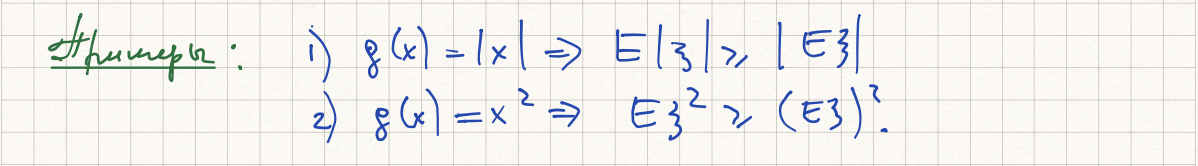
\includegraphics[width=1\textwidth]{sections/sasha/images/zbc-iensen-examples.png}